%%%%%%%%%%%%%%%%%%%%%%%%%%%%%%%%%%%%%%%%%%%%%%%%%%%%%%%%%%%%%%%%%%%%%%%%%%%%%%%%%%%%%%%%%%%%%%%%
%
% CS484 Written Question Template
%
% Acknowledgements:
% The original code is written by Prof. James Tompkin (james_tompkin@brown.edu).
% The second version is revised by Prof. Min H. Kim (minhkim@kaist.ac.kr).
%
% This is a LaTeX document. LaTeX is a markup language for producing 
% documents. Your task is to fill out this document, then to compile 
% it into a PDF document. 
%
% 
% TO COMPILE:
% > pdflatex thisfile.tex
%
% If you do not have LaTeX and need a LaTeX distribution:
% - Personal laptops (all common OS): www.latex-project.org/get/
% - We recommend latex compiler miktex (https://miktex.org/) for windows,
%   macTex (http://www.tug.org/mactex/) for macOS users.
%   And TeXstudio(http://www.texstudio.org/) for latex editor.
%   You should install both compiler and editor for editing latex.
%   The another option is Overleaf (https://www.overleaf.com/) which is 
%   an online latex editor.
%
% If you need help with LaTeX, please come to office hours. 
% Or, there is plenty of help online:
% https://en.wikibooks.org/wiki/LaTeX
%
% Good luck!
% Min and the CS484 staff
%
%%%%%%%%%%%%%%%%%%%%%%%%%%%%%%%%%%%%%%%%%%%%%%%%%%%%%%%%%%%%%%%%%%%%%%%%%%%%%%%%%%%%%%%%%%%%%%%%
%
% How to include two graphics on the same line:
% 
% \includegraphics[width=0.49\linewidth]{yourgraphic1.png}
% \includegraphics[width=0.49\linewidth]{yourgraphic2.png}
%
% How to include equations:
%
% \begin{equation}
% y = mx+c
% \end{equation}
% 
%%%%%%%%%%%%%%%%%%%%%%%%%%%%%%%%%%%%%%%%%%%%%%%%%%%%%%%%%%%%%%%%%%%%%%%%%%%%%%%%%%%%%%%%%%%%%%%%

\documentclass[11pt]{article}

\usepackage[english]{babel}
\usepackage[utf8]{inputenc}
\usepackage[colorlinks = true,
            linkcolor = blue,
            urlcolor  = blue]{hyperref}
\usepackage[a4paper,margin=1.5in]{geometry}
\usepackage{stackengine,graphicx}
\usepackage{fancyhdr}
\setlength{\headheight}{15pt}
\usepackage{microtype}
\usepackage{times}
\usepackage{booktabs}

% From https://ctan.org/pkg/matlab-prettifier
\usepackage[numbered,framed]{matlab-prettifier}

\frenchspacing
\setlength{\parindent}{0cm} % Default is 15pt.
\setlength{\parskip}{0.3cm plus1mm minus1mm}

\pagestyle{fancy}
\fancyhf{}
\lhead{Project Writeup}
\rhead{CS 484}
\rfoot{\thepage}

\date{}

\title{\vspace{-1cm}Homework 4 Writeup}


\begin{document}
\maketitle
\vspace{-3cm}
\thispagestyle{fancy}

\section*{Instructions}
\begin{itemize}
  \item Describe any interesting decisions you made to write your algorithm.
  \item Show and discuss the results of your algorithm.
  \item Feel free to include code snippets, images, and equations.

\end{itemize}

\section*{get\_interest\_point}

I approximated the gradient of image by applying sobel filter. From the gradient, I could get the second momentum matrix M. I computed the determinant and trace of M. $C = det(M) - \alpha * trace(M)^2$, and if C is greater than threshold, which I decided as 0.006, the point represent corner. 

\section*{get\_descriptors}

I first padded the image to avoid using zero pixel values for window when finding descriptors for pixel close to the end of image. Then for the given pixel, I retrieved surrounding window's derivatives, x and y direction each. From the derivatives, the histogram for edge direction can be found, to get the major direction shown in the window. Using the direction, Total direction of the window is normalized to get orientation invariance. Local histogram is formed using the normalized directions, and the feature of the point is formed using each of the local histograms. 16 locals are formed from the window, and histogram is formed by dividing angle into 8 partitions, so that the dimension of the feature is 16*8 = 128. The feature is normalized, and any value over 0.2 got fixed to 0.2 to avoid error from specular point. The feature get normalized again, and the stack of features for all the given points get returned.

\section*{match\_features}
For a given two features, the difference is computed. I used cosine difference, which is 1 - (cosine similarity) as the feature represent angular values. For a point on one image, I found 2 matching points on the other image, point with most closest feature and second closest feature. Then the difference between features is compared. If the ratio of difference, (distance to most closest point)/(distance to second closest point), is less than threshold, which I choose as 0.75, the most closest point is decided to match with the given point. The match point pairs and confidence, (distance to second closest point)(distance to most closest point) is returned. 

\begin{figure}[h]
    \centering
    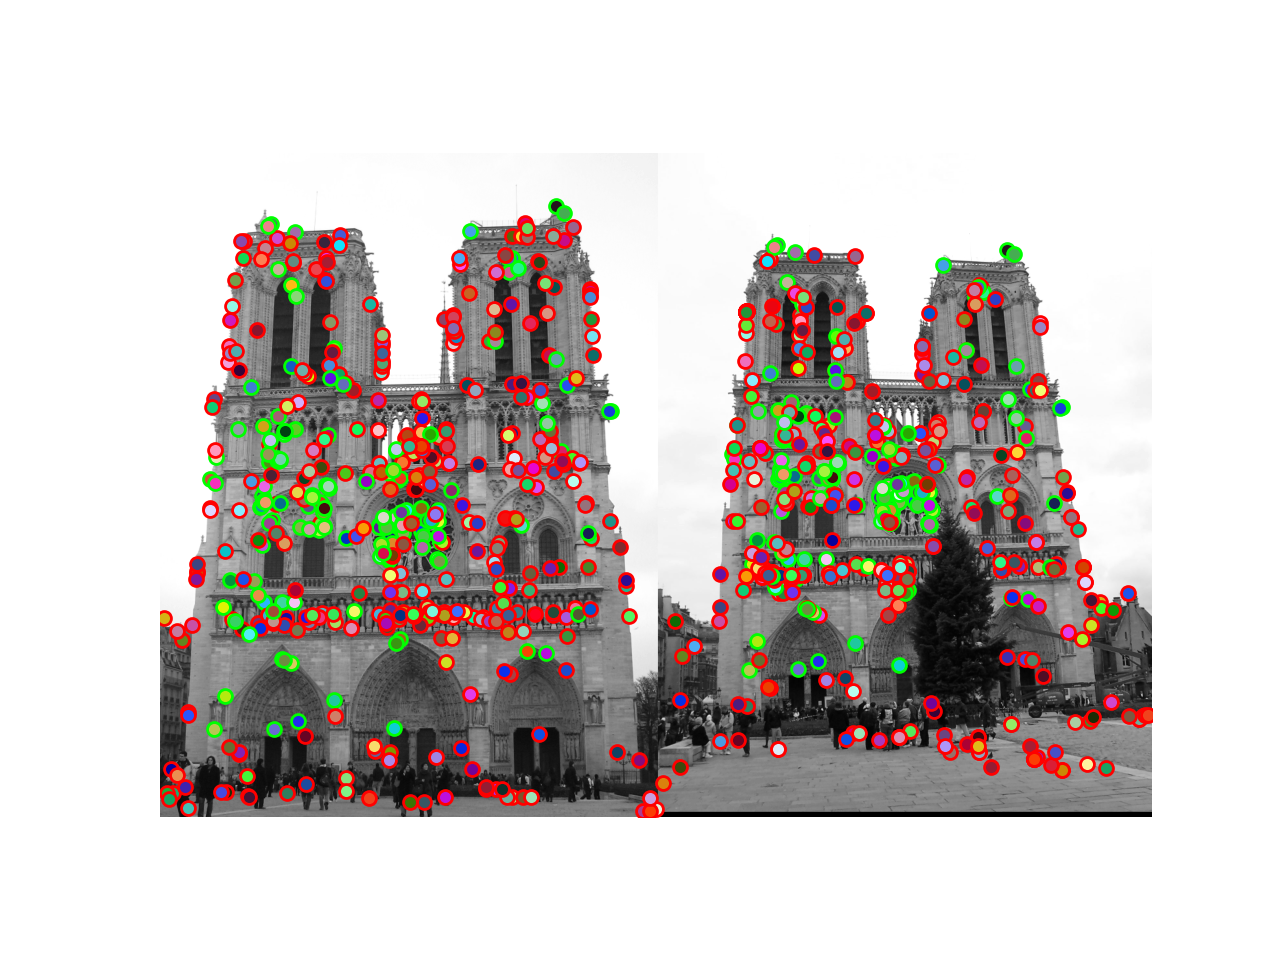
\includegraphics[width=10cm]{../code/eval_ND.png}
    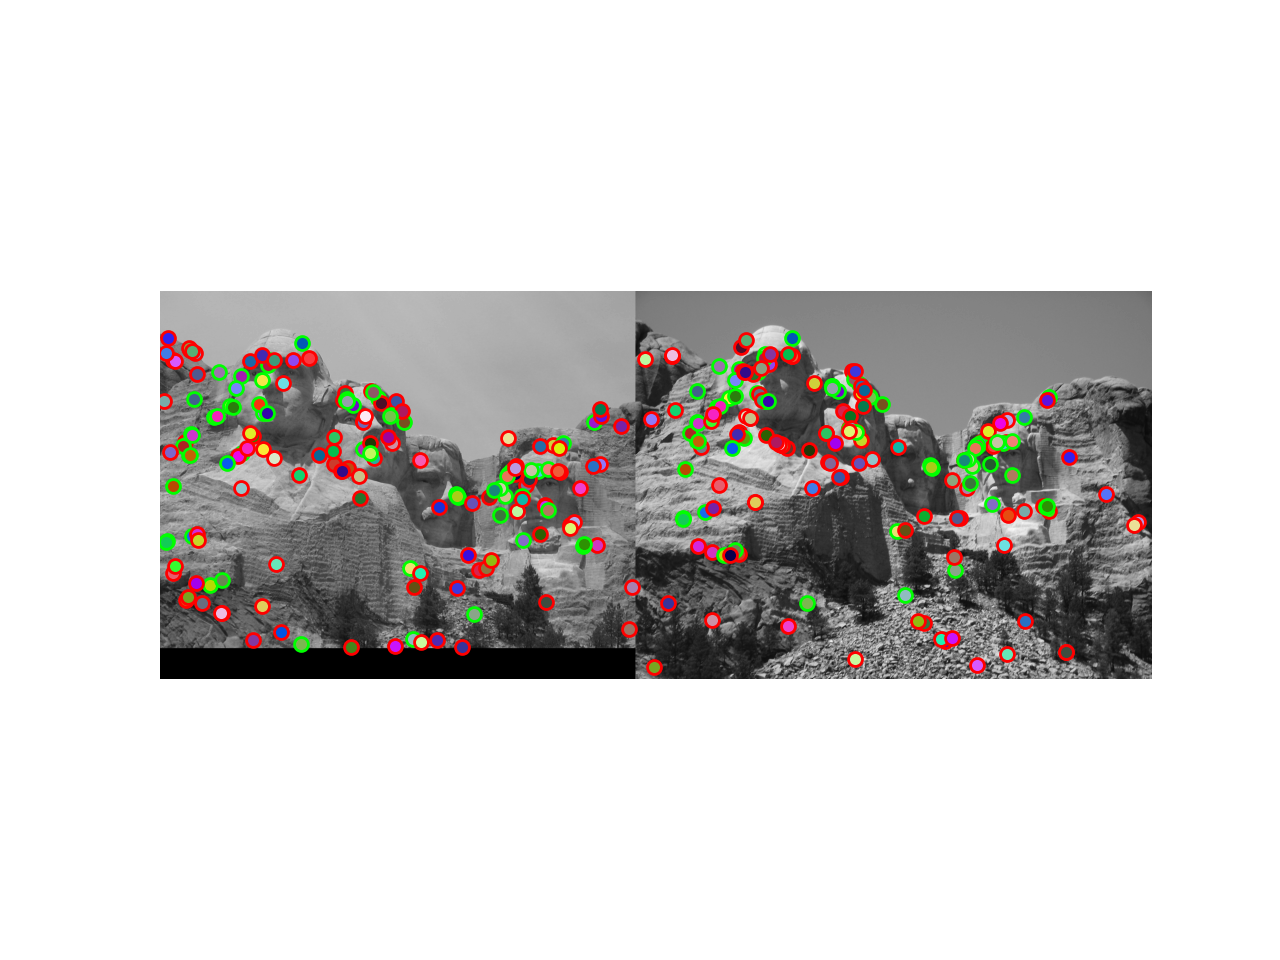
\includegraphics[width=10cm]{../code/eval_MR.png}
    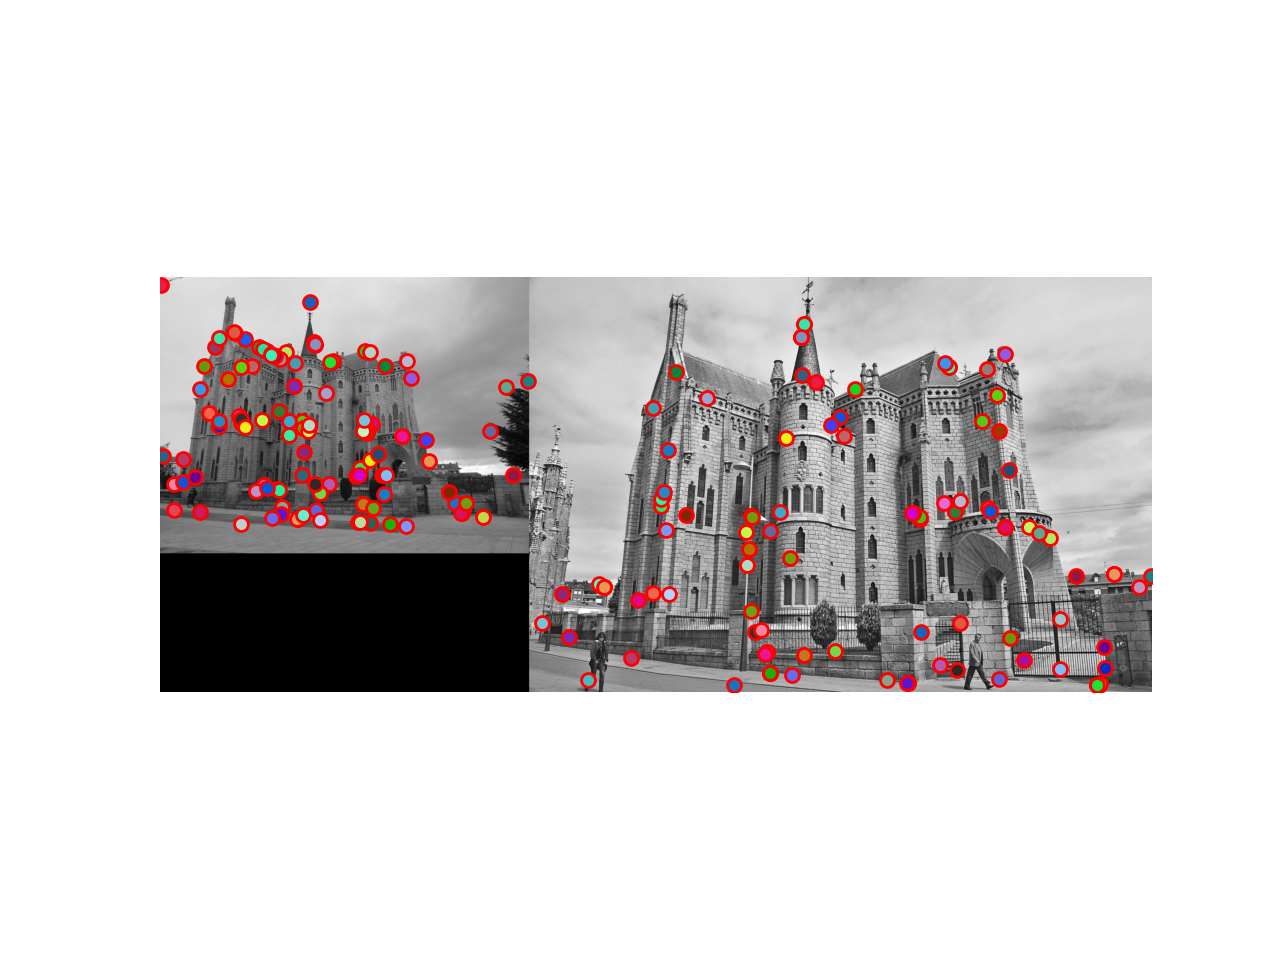
\includegraphics[width=10cm]{../code/eval_EG.png}
    \label{feature points for the given images}
\end{figure}


\end{document}
